\chapter{A história e a queda do dinheiro}
\label{les:12}

\begin{chapquote}{Lewis Carroll, \textit{Alice no País das Maravilhas}}
\enquote{tudo porque não se lembravam das regrinhas simples que seus amigos lhes haviam ensinado: que um atiçador em brasa acaba queimando sua mão se você insistir em segurá-lo por muito tempo; quando você corta o dedo muito fundo com uma faca, geralmente sai sangue;e ela nunca esquecera que, se você bebe muito de uma garrafa em que está escrito “veneno”, é quase certo que vai se sentir mal, mais cedo ou mais tarde.}
\end{chapquote}

Muitas pessoas pensam que o dinheiro é lastreado em ouro, que está trancado em grandes cofres enterrado bem fundo no subterrâneo do banco central do país, protegido por paredes grossas. Isso deixou de ser verdade há muitas décadas. Não tenho certeza do que pensei, uma vez que estava em apuros bem sérios, não tendo virtualmente nenhuma compreensão de ouro, papel-moeda ou por que ele precisaria ser lastreado por algo em primeiro lugar.

Uma parte de aprender sobre o Bitcoin é aprender sobre a moeda fiduciária: o que significa, como surgiu e por que pode não ser a melhor ideia que já tivemos. Então, o que exatamente é a moeda fiduciária? E como acabamos usando isso?

Se algo é imposto \textit{fiduciariamente}, significa simplesmente que é imposto por autorização ou proposição formal. Assim, a moeda fiduciária é dinheiro simplesmente porque \textit{alguém} disse que é dinheiro. Como todos os governos usam moeda fiduciária hoje, esse alguém é \textit{seu} governo. Infelizmente, você não está \textit{livre} para discordar desta proposta de valor. Você sentirá rapidamente que essa proposição é tudo, menos pacífica. Se você se recusar a usar esse papel-moeda para fazer negócios e pagar impostos, as únicas pessoas com quem você poderá discutir sobre economia serão seus colegas de cela.

O valor da moeda fiduciária não decorre de suas propriedades inerentes. O quão bom é uma moeda fiduciária, está relacionado a, única e exclusivamente, sua capacidade de ter (in)estabilidade política e fiscal daqueles que sonham com sua existência. Seu valor é imposto por decreto, de forma arbitrária.

\begin{figure}
  \centering
  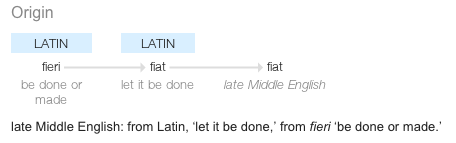
\includegraphics[width=8cm]{assets/images/fiat-definition.png}
  \caption{Fiat --- `Deixe ser feito'}
  \label{fig:fiat-definition}
\end{figure}

\paragraph{}
Até recentemente, dois tipos de dinheiro eram usados: \textbf{moeda-mercadoria}, feita com \textit{coisas} preciosas, e \textbf{dinheiro representativo}, que simplesmente \textit{representa} o que é precioso, principalmente na escrita.

\paragraph{}
Já tocamos na moeda-mercadoria acima. As pessoas usavam ossos especiais, conchas e metais preciosos como dinheiro. Mais tarde, principalmente moedas feitas de metais preciosos como ouro e prata foram usadas como dinheiro. A moeda mais antiga encontrada até agora é feita de uma mistura natural de ouro e prata e foi feita há mais de 2.700 anos. \Footnote{De acordo com o historiador grego Heródoto, que escreveu no século V AC, os lídios foram os primeiros a usaram moedas de ouro e prata. \cite{coinage-origins}} Se algo é novo no Bitcoin, o conceito de moeda não é isso.

\begin{figure}
  \centering
  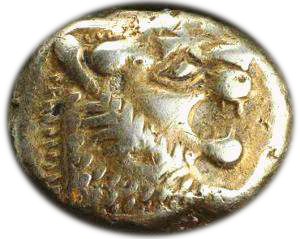
\includegraphics[width=5cm]{assets/images/lydian-coin-stater.png}
  \caption{Uma moeda da Lídia. Imagem sob licença cc-by-sa da Classical Numismatic Group, Inc.}
  \label{fig:lydian-coin-stater}
\end{figure}

Acontece que acumular moedas, ou hodling, para usar o jargão atual, é quase tão antigo quanto as moedas da antiguidade. O primeiro criador de moedas foi alguém que colocou quase uma centena dessas moedas em um pote e as enterrou nas fundações de um templo, apenas para ser encontrado 2500 anos depois. Um armazenamento frio (também conhecido pelo jargão inglês de Cold Storage) muito bom, se você me perguntar.

Uma das desvantagens de se usar as moedas de metal precioso é que elas podem ser cortadas, efetivamente degradando o valor da moeda. Novas moedas podem ser cunhadas a partir dos pedaços, inflando a oferta de dinheiro ao longo do tempo, desvalorizando cada moeda individual no processo. As pessoas estavam literalmente cortando o máximo que podiam das suas moedas de dólares de prata. Eu me pergunto que tipo de anúncio de \textit{Clube das Tesouras} eles tinham naquela época.

Uma vez que os governos só ficam calmos com a inflação se são eles que a praticam, esforços foram feitos para impedir essa depreciação pelos cidadãos. No clássico estilo de polícia e ladrão, os depreciadores de moedas ficaram cada vez mais criativos com suas técnicas, forçando os \enquote{mestres da cunhagem} a ficarem ainda mais criativos em suas contra-medidas. Isaac Newton, o mundialmente conhecido físico que escreveu o livro \textit{Principia Mathematica}, costumava ser um desses mestres. Ele quem adicionou pequenas listras ao lado das moedas que ainda estão presentes hoje. Já se foram os dias em que era fácil depreciar as moedas.

\begin{figure}
  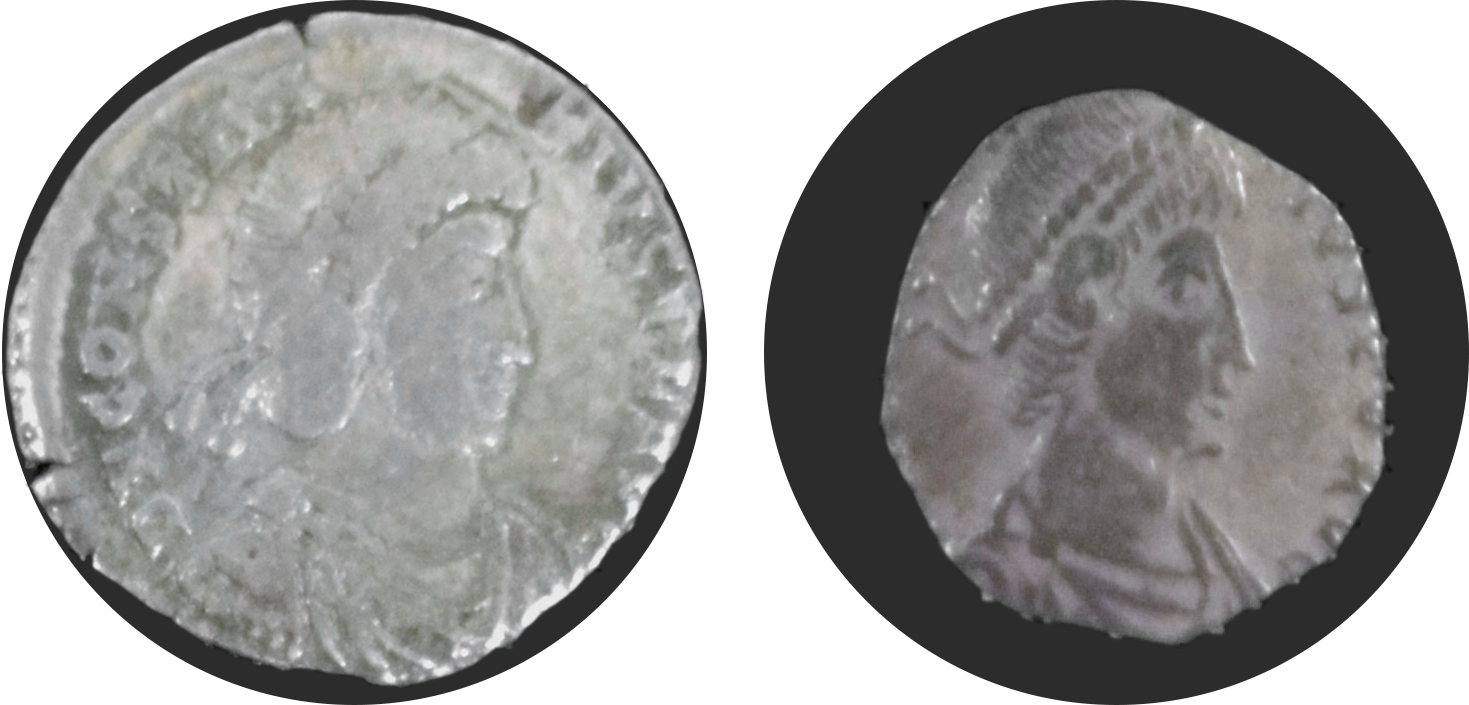
\includegraphics{assets/images/clipped-coins.png}
  \caption{Moedas de prata com cortes de tamanhos variados.}
  \label{fig:clipped-coins}
\end{figure}

Mesmo com esses métodos de depreciação das moedas \footnote{Além de recortar, dissolver (sacudir as moedas em um saco e coletar o seu pó) e tamponar (retirar o miolo da moeda fazendo um furo e depois, martelar a moeda até fechá-lo) foram os métodos mais utilizados para depreciar as moedas. \cite{wiki:coin-debasement}} mantidos sob controle, as moedas ainda sofrem de outros problemas. Elas são volumosas e não são muito convenientes para transportar, especialmente quando grandes transferências de valor precisam acontecer. Aparecer com uma enorme sacola de dólares de prata toda vez que você quiser comprar uma Mercedes não é algo muito prático.

Falando de coisas alemãs: como os \textit{dólares} dos Estados Unidos ganharam esse nome é outra história interessante. A palavra \enquote{dólar} é derivada da palavra alemã \textit{Thaler}, abreviação de \textit{Joachimsthaler}~\cite{wiki:thaler}. Um Joachimsthaler foi uma moeda cunhada na cidade de \textit{Sankt Joachimsthal}. O Thaler é simplesmente uma abreviatura para alguém (ou algo) vindo do vale, e porque Joachimsthal era \textit{o} vale da produção de moedas de prata, as pessoas simplesmente se referiam a essas moedas de prata como \textit{Thaler}. O Thaler (alemão) se transformou em daalders (holandês) e, finalmente, dólares (inglês).

\begin{figure}
  \centering
  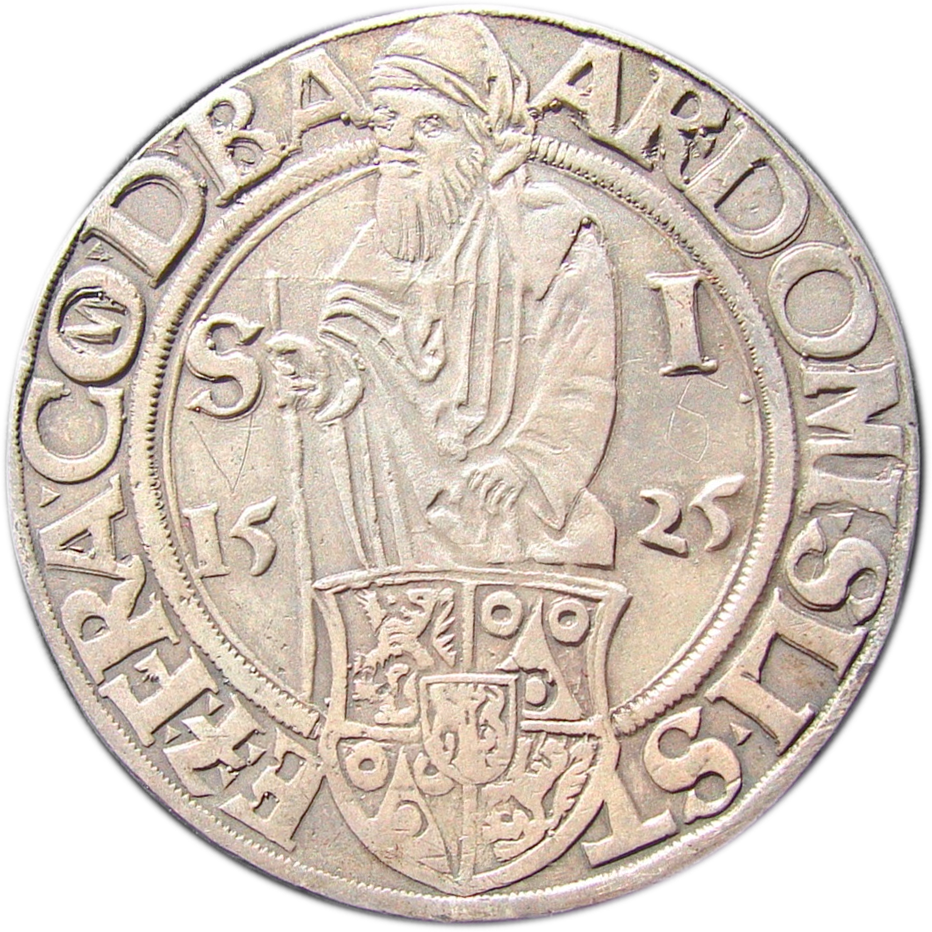
\includegraphics[width=5cm]{assets/images/joachimsthaler.png}
  \caption{O 'Dólar' original. Saint Joachim foi colocado na face da mooeda com seu manto e seu chapéu de mago. A imagem está sob licença cc-by-sa da Wikipedia enviada pelo usuário Berlin-George}
  \label{fig:joachimsthaler}
\end{figure}

A introdução do dinheiro representativo foi o prenúncio da queda do dinheiro forte. Os certificados de ouro foram introduzidos em 1863 e, cerca de quinze anos depois, o dólar de prata também foi lenta, mas constantemente, sendo substituído por uma procuração em papel: o certificado de prata. \cite{wiki:silver-certificate}

Demorou cerca de 50 anos desde a introdução dos primeiros certificados de prata até que esses pedaços de papel se transformassem em algo que hoje reconheceríamos como um dólar americano.

\begin{figure}
  \centering
  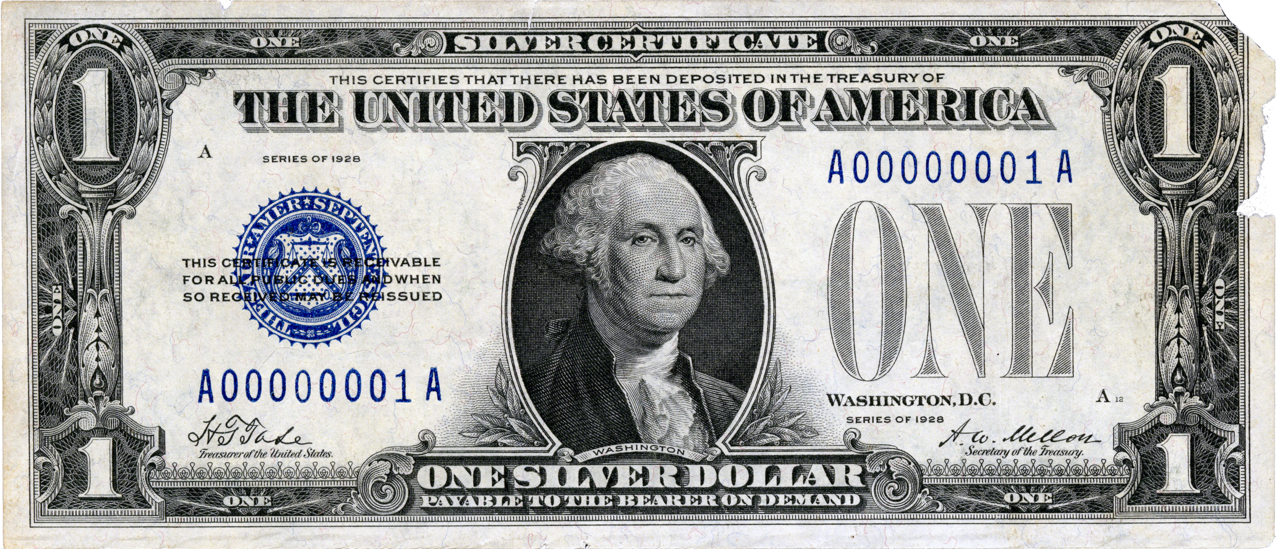
\includegraphics{assets/images/us-silver-dollar-note-smaller.png}
  \caption{Um dólar americano de 1928. `Pagável ao portador sob demanda.' A imagem está sob licença cc-by-sa publicada pela National Numismatic Collection at the Smithsonian Institution}
  \label{fig:us-silver-dollar-note-smaller}
\end{figure}

Observe que o dólar de prata dos EUA de 1928 na Figura ~\ref{fig:us-silver-dollar-note-smaller} ainda atende pelo nome de \textit{certificado de prata}, indicando que este é de fato simplesmente um documento afirmando que o portador deste pedaço de papel tem direito a uma moeda de prata. É interessante ver que o texto que indica isso foi ficando menor com o tempo. O traço do \enquote{certificado} desapareceu completamente depois de um tempo, sendo substituído pela declaração tranquilizadora de que essas são notas do Federal Reserve.

Como mencionado acima, o mesmo aconteceu com o ouro. A maior parte do mundo seguia um padrão bimetálico ~\cite {wiki:bimetallism}, o que significa que as moedas eram feitas principalmente de ouro e prata. Ter certificados de ouro, resgatáveis em moedas de ouro, era indiscutivelmente uma melhoria tecnológica. O papel é mais conveniente, mais leve e, como pode ser dividido arbitrariamente, simplesmente imprimindo um número menor nele, é mais fácil dividi-lo em unidades menores.

Para lembrar aos portadores (usuários) que esses certificados eram representativos do ouro e da prata reais, eles tinham cores de acordo com o metal e isso era declarado claramente no próprio certificado. Você pode ler com facilidade a escrita de cima para baixo:

\begin{quotation}\begin{samepage}
\enquote{Isso certifica que foram depositados no tesouro dos Estados Unidos da América cem dólares em moedas de ouro pagáveis ao portador à vista.}
\end{samepage}\end{quotation}

\begin{figure}
  \centering
  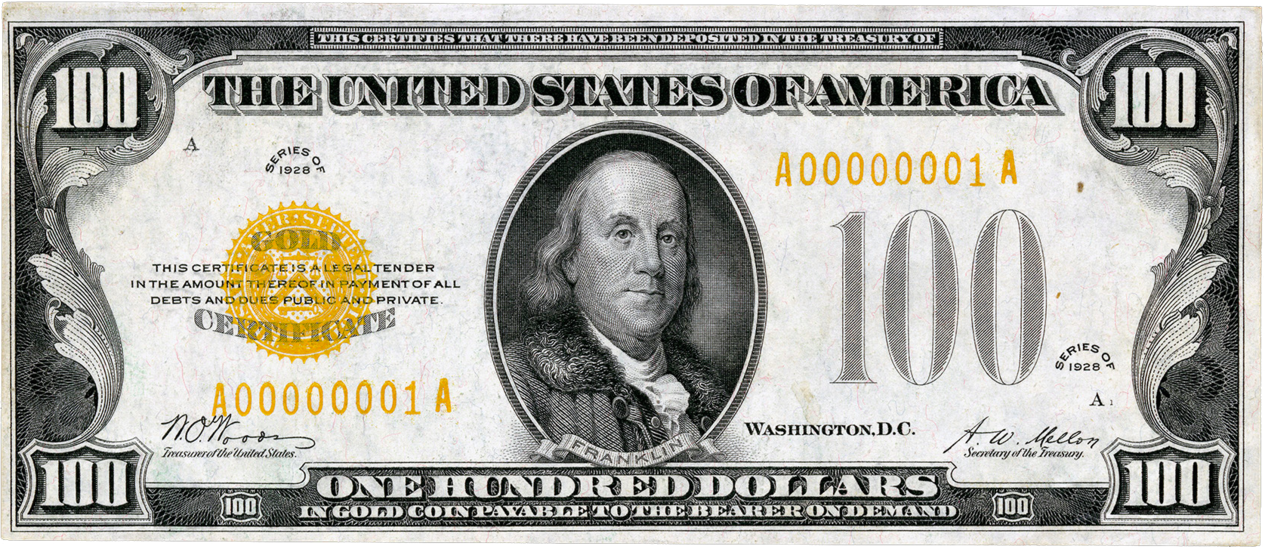
\includegraphics{assets/images/us-gold-cert-100-smaller.png}
  \caption{Uma note de \$100 dólares cunhada em 1928 em certificados de ouro. A imagem está sob licença cc-by-sa publicada pela National Numismatic Collection, National Museum of American History.}
  \label{fig:us-gold-cert-100-smaller}
\end{figure}

Em 1963, as palavras \enquote{APAGAR AO PORTADOR SOB DEMANDA} foram removidas de todas as notas recém-emitidas. Cinco anos depois, o resgate das notas de papel por ouro e prata terminou.

As palavras que sugeriam as origens e a ideia por trás do papel-moeda foram removidas. A cor dourada desapareceu. Tudo o que restou foi o papel e com ele a capacidade do governo de imprimir o quanto quiser.

Com a abolição do padrão-ouro em 1971, esse truque de prestidigitação secular estava finalizado. O dinheiro se tornou a ilusão que todos compartilhamos até hoje: um dinheiro fiduciário. Vale alguma coisa porque alguém comandando um exército e operando prisões diz que vale alguma coisa. Como pode ser lido claramente em cada nota de dólar em circulação hoje, \enquote{ESTA NOTA É DE CURSO LEGAL}. Em outras palavras: é valiosa porque a nota diz que ela é valiosa.

\begin{figure}
  \centering
  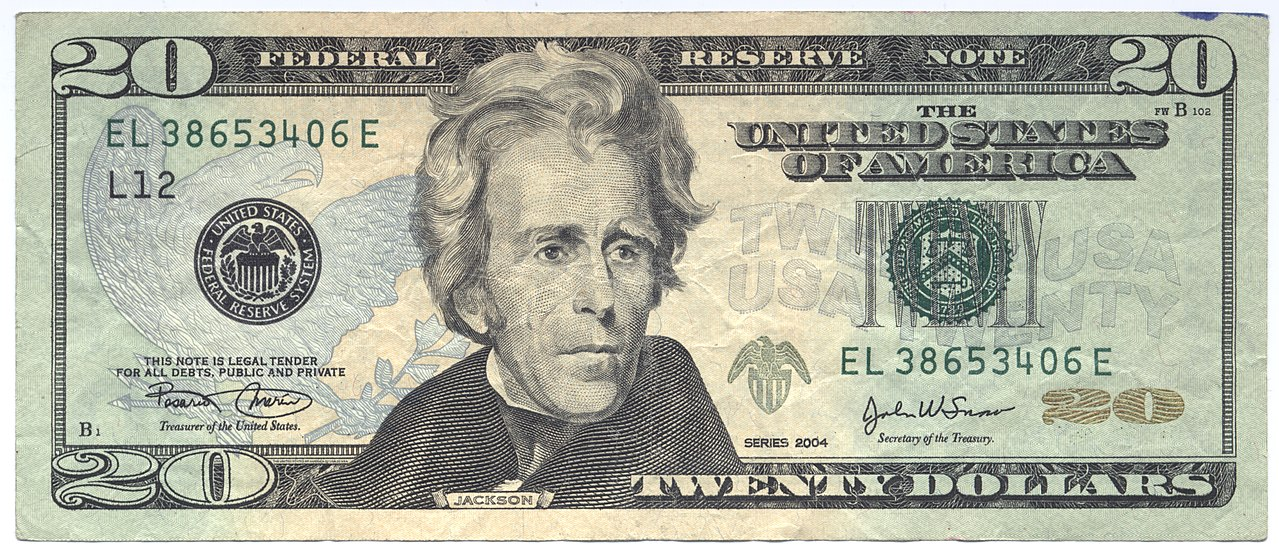
\includegraphics{assets/images/us-dollar-2004.jpg}
  \caption{Uma nota de vinte dólares americanos de 2004 usada atualmente. `ESTA NOTA É DE CURSO LEGAL'}
  \label{fig:us-dollar-2004}
\end{figure}

A propósito, há outra lição interessante sobre as notas de hoje, que está escondido mas ao mesmo tempo estampado na cara de todo mundo. A segunda linha diz que ela é de curso legal \enquote{PARA TODAS AS DÍVIDAS, PÚBLICAS E PRIVADAS}. O que pode ser óbvio para os economistas, me surpreendeu: todo dinheiro é dívida. Minha cabeça ainda está doendo por causa disso, e deixarei a exploração da relação entre dinheiro e dívida como um exercício para você, leitor.

\paragraph{}
Como vimos, ouro e prata foram usados como dinheiro por milênios. Com o tempo, as moedas feitas de ouro e prata foram substituídas por papel. O papel foi lentamente sendo aceito como forma de pagamento. Essa aceitação criou uma ilusão - a ilusão de que o próprio papel tem valor. O movimento final foi cortar completamente o vínculo entre a representação e o seu valor real: abolindo o padrão-ouro e convencendo a todos de que o papel em si é precioso.

\paragraph{O Bitcoin me ensinou sobre a história do dinheiro e o maior truque da história da economia: a moeda fiduciária.}

% ---
%
% #### Down the Rabbit Hole
%
% - [Shelling Out: The Origins of Money] by Nick Szabo
% - [Methods of Coin Debasement][coin debasement], [Thaler], [U.S. Silver Certificate][silver certificates], [Bimetallism][bimetallic standard] on Wikipedia
%
% [oldest coin]: https://www.britishmuseum.org/explore/themes/money/the_origins_of_coinage.aspx
% [coin debasement]: https://en.wikipedia.org/wiki/Methods_of_coin_debasement
% [Thaler]: https://en.wikipedia.org/wiki/Thaler
% [Berlin-George]: https://en.wikipedia.org/wiki/File:Bohemia,_Joachimsthaler_1525_Electrotype_Copy._VF._Obverse..jpg
% [silver certificates]: https://en.wikipedia.org/wiki/Silver_certificate_%28United_States%29
% [bimetallic standard]: https://en.wikipedia.org/wiki/Bimetallism
% [Shelling Out: The Origins of Money]: https://nakamotoinstitute.org/shelling-out/
%
% <!-- Wikipedia -->
% [alice]: https://en.wikipedia.org/wiki/Alice%27s_Adventures_in_Wonderland
% [carroll]: https://en.wikipedia.org/wiki/Lewis_Carroll
